\documentclass[onecolumn]{article}
\usepackage{graphicx}
\usepackage{float}
\usepackage{hyperref}
\restylefloat{figure}
\begin{document}

\title{One-dimensional diffusion-reaction equation and "water age"}

\author{Arjen Markus}

\maketitle

\section*{Introduction}
In environmental studies of, say, a reservoir or an estuary it is often useful to determine characteristic or diagnostic
timescales that allow you to reason about the refreshment of the water in the system. It makes quite a difference to
the dynamics of a water system if the time to refresh most of the water is several days or several years. One way to
determine such timescales, and this is only one, is to use tracers in a numerical model.\footnote{An alternative
method is CART, Constituent-oriented Age and Residence time Theory, \url{http://www.climate.be/cart}.}
 The transport of these
tracers by flow or by mixing processes as calculated by the model is then analysed to produce an estimate of the timescale
of interest. Simply put: fill the model with a passive (conservative) tracer such that the concentration is, say, 1~mg/l, let
the boundary concentration be zero and determine how fast the average concentration decreases. This will give you an idea
of the refreshment of the water in the overall system.

This can be put into a more sophisticated form by using two tracers, one conservative and one decaying slowly (like a radio-active
substance would), and determining the so-called "radio age":
\begin{eqnarray}
\label{radioage}
    T_{radio} &=& -\frac{1}{k} \ln \frac{C_{decaying}}{C_{conservative}}
\end{eqnarray}
%
\noindent where $k$ is the decay coefficient of the decaying tracer. This way, you get a detailed estimate of the time the
tracers have been in the system: spatial variation as well as temporal variation.

In this note I want to examine an idealised situation from a mathematical point of view. The reason is that the technique I
used, while hardly new and while none of the results are new, Laplace transforms, gave me a surprise. I knew something was
wrong with my first attempt, but I could not figure out what. As in most publications the solutions are simply cited without
any derivation, I thought it might be useful to write down my mistakes.

%TODO:
%
%Mention CART. I could do the same analysis based on CART, but that poses another surprise ...

\section*{The problem at hand: one-dimensional diffusion-reaction}
The problem is a fairly classical one:

Consider an infinite channel (or a bar of some homogeneous material, if you think of heat conduction). At the origin there is either an instantaneous
release (in which case we let the channel run into two directions) or a boundary with a constant concentration of the
two tracers -- a continuous release as it were. There is no advection, only diffusion. One of the two tracers decays linearly with a rate $k$, the
other is conservative.

The equations are:
\begin{eqnarray}
\label{transport1}
    \frac{\partial C_c}{\partial t} &=& D \frac{\partial^2 C_c}{\partial x^2} \\
\label{transport2}
    \frac{\partial C_d}{\partial t} &=& D \frac{\partial^2 C_d}{\partial x^2} - k C_d
\end{eqnarray}
%
\noindent where $D$ is the diffusion coefficient.

The boundary conditions are:
\begin{itemize}
\item
For the instantaneous and the continuous release: $C_d, C_c$ remain finite as $|x| \rightarrow \infty$.
\item
For the instantaneous release: a mass $M$ is released at $x = 0$ -- represented as a $\delta$ function.
\item
For the continuous release: $C_d, C_c = 1$ for $x = 0$ (and $x \geq 0$).
\end{itemize}
In both cases the initial condition is: $C_d, C_c = 0$.

\section*{Limiting solutions}
If we let time go to infinity, then the solution is very simple:
\begin{itemize}
\item
For the instantaneous release the finite mass of both tracers will be spread out over the whole channel, so the
limiting solution is: $C_d, C_c = 0$.
\item
For the continuous release:
\begin{itemize}
\item
The concentration of the conservative tracer will become 1 for all $x \geq 0$.
\item
The concentration of the decaying tracer will become:
\begin{eqnarray}
    C_d = e^{-x \sqrt{k/D}}
\end{eqnarray}
\end{itemize}
Applying the definition of the radio age (Eq.\ \ref{radioage}):
\begin{eqnarray}
    T_{radio} &=& \frac{1}{k} (x \sqrt{k/D}) = \frac{x}{\sqrt{kD}}
\end{eqnarray}

In this case, the water age depends on both the diffusion coefficient and the decay coefficient, so it is not
a property of the water system alone, but more worrisome, if you were to let the decay coefficient go to zero,
the limit goes to infinity.
\end{itemize}

Note that if there is a steady flow (from left to right), the steady-state equation to solve becomes:
\begin{eqnarray}
      u \frac{dC_d}{dx} &=& D \frac{d^2C_d}{dx^2} - k C_d
\end{eqnarray}
\noindent with as a solution to the same boundary conditions:
\begin{eqnarray}
      C_d &=& e^{-\lambda x} \\
      \lambda &=& \frac{u}{2D} \bigl(\sqrt{1 + \frac{4 D k}{u^2}} - 1 \bigr)
\end{eqnarray}
\noindent so that the radio age becomes (for small $k$):
\begin{eqnarray}
\nonumber T_{radio} &=&       -\frac{1}{k} \lambda x \\
\nonumber      &\approx& -\frac{1}{k} \frac{u x}{2D} \bigl((1 + \frac{2 D k}{u^2}) - 1 \bigr) \\
\nonumber      &=&       \frac{1}{k} \frac{u x}{2D} \frac{2 D k x}{u^2} \\
               &=&       \frac{x}{u}
\end{eqnarray}

Thus, when there is a steady flow, the radio age (in the limit $k \rightarrow 0$) is equal to the travel time of the water,
whereas without flow the "age" depends on both the decay coefficient and the dispersion coefficient.


\section*{Full solutions}
Now let us concentrate on the full solutions, where the concentration depends on time and space.
The simplest way to find a solution is to use the Laplace transformation. Equations \ref{transport1} and \ref{transport2} then
become (the initial condition for both $C_c$ and $C_d$ is zero and the boundary conditions are constant):
\begin{eqnarray}
    s C_c &=& D \frac{d^2 C_c}{d x^2} \\
    s C_d &=& D \frac{d^2 C_d}{d x^2} - k C_d
\end{eqnarray}

These ordinary differential equations can easily be solved and then we need to find the inverse transform. The
solutions are:
\begin{eqnarray}
    C_c(x,s) &=& e^{-x \sqrt{s/D}} \\
    C_d(x,s) &=& e^{-x \sqrt{(s+k)/ D}}
\end{eqnarray}

With the aid of the site \url{https://www.wolframalpha.com/input/?i=inverse+Laplace+transform} we find the inverse
transform to be:
\begin{eqnarray}
    C_c(x,t) &=& \frac{x e^{-x^2/4Dt}}{2 \sqrt{\pi D} t^{3/2}}     \\
    C_d(x,t) &=& \frac{x e^{-kt -x^2/4Dt}}{2 \sqrt{\pi D} t^{3/2}}
\end{eqnarray}

And these solutions are wrong! They cannot be the solutions of the problem we want to solve:
\begin{itemize}
\item
The concentration at $x = 0$ is zero, not $1$.
\item
Examining the transformed solutions, we see that for $x = 0$ the value is constantly 1, for $s \geq 0$, and that is only possible
for a Laplace transform of the Dirac delta function.
\end{itemize}

I was puzzled, when I found these solutions and thought the inverse transforms were wrong, but that is not the
case: I forgot to properly transform the boundary conditions! They should read:
\begin{eqnarray}
    C_c, C_d = \frac{1}{s}, ~~~~x = 0
\end{eqnarray}
\noindent as the boundary conditions are also subject to the Laplace transformation.

With that realisation, we can now obtain the correct transformed solutions:
\begin{eqnarray}
    C_c(x,s) &=& \frac{1}{s} e^{-x \sqrt{s/D}} \\
    C_d(x,s) &=& \frac{1}{s} e^{-x \sqrt{(s+k)/ D}}
\end{eqnarray}

The inverse transforms of the above two solutions are:
\begin{eqnarray}
\nonumber    C_c(x,t) &=& \textrm{erfc} \bigl(\frac{x}{2 \sqrt{Dt}} \bigr) \\
\nonumber    C_d(x,t) &=& \frac{1}{2} e^{-\sqrt{k/D}~x} \Bigl( \textrm{erf} \bigl(\frac{2\sqrt{k/D}~t -x}{2 \sqrt{t}} \bigr) + \\
                      & &             ~~~~~ e^{2 \sqrt{k/D}~x} \textrm{erfc} \bigl(\frac{2 \sqrt{k/D}~t + x} {2 \sqrt{t}} \bigr) + 1 \Bigr)
\end{eqnarray}

Of course, the formulae are rather intractable when it comes to determining the radio age as a function of time and space and that is
a bit of a pity.


\begin{figure}[H]
\caption{Concentration of the conservative and decaying tracers for different times.}
\label{conservative_decaying}
\begin{center}
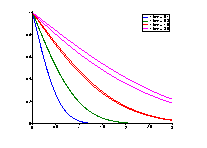
\includegraphics[width=0.7\textwidth]{conservative_decaying.pdf}
\end{center}
\end{figure}

\begin{figure}[H]
\caption{Estimated age based on the conservative and decaying tracers for different times.}
\label{estimated_age}
\begin{center}
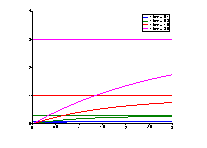
\includegraphics[width=0.7\textwidth]{estimated_age.pdf}
\end{center}
\end{figure}




\section*{Sanity check}
The solutions may consist of rather complicated expressions, but we can check that they make sense: the estimated age should not
exceed the time in the solutions. So, by plotting the curves for several values of time $t$ and also plotting the estimated age
we can at least informally check this condition. The result is shown in the two figures.

The "age" of the tracers is zero at the left boundary and increases in the positive x-direction to the time $t$. This is as expected.
At the left boundary the tracers enter the system and it takes time to reach the other side.


\section*{Conclusion}
While the Laplace transform, in combination with online services to get the inverse, is a really useful tool for solving these partial
differential equations, you need to be careful to transform the complete set of equations: not only the equations themselves, but
also the relevant boundary conditions.


%\begin{eqnarray}
%Laplace = e^{-x \sqrt{s+k}} &\rightarrow& \frac{x e^{-kt -x^2/4t}}{2 \sqrt{\pi} t^{3/2}}
%\end{eqnarray}
%\begin{eqnarray}
%Laplace = \frac{1}{s} e^{-x \sqrt{s}} &\rightarrow& \textrm{erfc} \bigl(\frac{x}{2 \sqrt{t}} \bigr)
%\end{eqnarray}
%\begin{eqnarray}
%Laplace = \frac{1}{s} e^{-x \sqrt{s+k}} &\rightarrow&
%     \frac{1}{2} e^{-\sqrt{k}~x} \Bigl( \textrm{erf} \bigl(\frac{2\sqrt{k}~t -x}{2 \sqrt{t}} \bigr) +
%                                        e^{2 \sqrt{k}~x} \textrm{erfc} \bigl(\frac{2 \sqrt{k}~t + x} {2 \sqrt{t}} \bigr) + 1 \Bigr)
%\end{eqnarray}
%Note: no D in there yet - x, k and t dimensionless.
\end{document}

